\documentclass[a4paper, 14pt]{extarticle}
\usepackage[T2A]{fontenc}
\usepackage[utf8]{inputenc}
\usepackage[russian]{babel}
\usepackage{geometry, amsmath, amssymb, mathtext, graphicx, caption,subfig, setspace, titlesec}
\geometry{left=3cm, right=1.5cm, top=2cm, bottom=2cm}

\captionsetup[figure]{labelsep=endash, justification=centering, name=Рисунок}

\onehalfspacing
\setlength{\parindent}{1.25cm}

\titleformat{\section}{\newpage\centering\normalfont\bfseries\large}{\thesection}{1em}{}
\titleformat{\subsection}{\normalfont\normalsize\bfseries}{\thesubsection}{1em}{}
\addto\captionsrussian{\renewcommand{\contentsname}{СОДЕРЖАНИЕ}}

\begin{document}
	
	\begin{titlepage}
		\centering
		{ Министерство науки и высшего образования Российской Федерации\\
		ФЕДЕРАЛЬНОЕ ГОСУДАРСТВЕННОЕ АВТОНОМНОЕ \\
		ОБРАЗОВАТЕЛЬНОЕ УЧРЕЖДЕНИЕ ВЫСШЕГО ОБРАЗОВАНИЯ \\
		<<МОСКОВСКИЙ ФИЗИКО-ТЕХНИЧЕСКИЙ ИНСТИТУТ\\
		(НАЦИОНАЛЬНЫЙ ИССЛЕДОВАТЕЛЬСКИЙ УНИВЕРСИТЕТ)>>\\
		(МФТИ,Физтех)
		}
		
		\vspace{6cm}
		
		КАФЕДРА ЭЛЕКТРОНИКИ\\
		\vspace{0.5cm}
		ОТЧЁТ \\
		ПО ЛАБОРАТОРНОЙ РАБОТЕ\\
		\vspace{0.5cm}
		{{ТЕРМОЭЛЕКТРОННЫЙ ДИОД}\\}
		
		\vspace{5cm}
		
		\begin{tabular}{ll}
			Работу выполнил & \underline{\hspace{5cm}} П.А. Рудачихин \\
			&\\
			Работу принял, оценка & \underline{\hspace{9cm}} \\
		\end{tabular}
		\centering
		
		
		\vfill
		
		Долгопрудный, 2026
	\end{titlepage}
	
	\section*{РЕФЕРАТ}
	\addcontentsline{toc}{section}{РЕФЕРАТ}
	
	\hspace{11mm} Отчёт  с.,  рис.,  табл.,  источн.
	
	ТЕРМОЭЛЕКТРОННЫЙ ДИОД, ТЕРМОЭЛЕКТРОННАЯ ЭМИССИЯ, ОБЪЁМЫЙ ЗАРЯД, ВОЛЬТ-АМПЕРНАЯ ХАРАКТЕРИСТИКА
	
	Объектом исследования является термоэлектронный диод.
	
	Цель настоящей работы -- практическое изучение явления термоэлектронной эмиссии и процессов токопрохождения в вакууме, изготовление вакуумного диода и исследование некоторых его характеристик. 
	
	В процессе работы проводилось изготовление диода и снятие его вольт-амперной характеристики при разных значениях температуры катода.	В результате ...
	
	
	\tableofcontents
	
	
	\section*{ВВЕДЕНИЕ}
	\addcontentsline{toc}{section}{ВВЕДЕНИЕ}
	
	\hspace{11mm} Термоэлектронной эмиссией (ТЭЭ) называют испускание электронов поверхностью нагретых проводящих тел. 
	
	Явление ТЭЭ и токопрохождение в вакууме лежат в основе работы многих электровакуумных приборов: радиоламп, приборов сверхвысоких частот, электронно-лучевых приборов. 
	
	От эмиссионной способности катодов зависит и режима токопрохождения зависят, например, мощность, широкополосность, шумовые характеристики и срок службы прибора. Поэтому изучение законов термоэлектронной эмиссии и токопрохождения в вакууме -- важная задача электроники. 
	
	В данной работе для изучения вышеперечисленных закономерностей создан и использован диод. Несмотря на то, что современные приборы сильно отличаются от диода, многие их характеристики подчиняются тем же закономерностям и рассчитываются теми же методами.
	
	Цель работы --- практическое изучение явления термоэлектронной эмиссии и процессов токопрохождения в вакууме, изготовление вакуумного диода и исследование некоторых его характеристик.
	
	В работе решаются следующие задачи:
	
	\begin{enumerate}
		\item Изготовить диод.
		\item Измерить зависимость напряжения накала от тока накала.
		\item Измерить зависимость анодного тока от анодного напряжения при разных токах накала.
		\item Определить первеанс и сравнить с расчётным.
		\item Вычислить удельный заряд электрона.
		\item Вычислить КПД диода для каждого значения тока накала.
	\end{enumerate}
	
	Объект исследования --- термоэлектронный диод.
	
	
	Методы исследования: построение вольт-амперной характеристики.
	
	
	\section{ТЕОРИЯ ТЕРМОЭЛЕКТРОННОЙ ЭМИССИИ}

	\hspace{11mm} Рассмотрим простейший прибор для наблюдения термоэлектронной эмиссии (ТЭЭ) -- термоэлектронный диод. Характерная особенность его вольт-амперной характеристики (см. рис. 1) -- от начала до точки перегиба ВАХ для разных температур катода совпадают, а после перегиба выходят на насыщение. На первом участке ток ограничен только потенциалом анода. На втором -- почти не зависит от потенциала анода, но явно зависит от температуры катода. Чтобы объяснить такое поведение, обратимся к теории.
	
	\begin{figure}[h!]
		\centering
		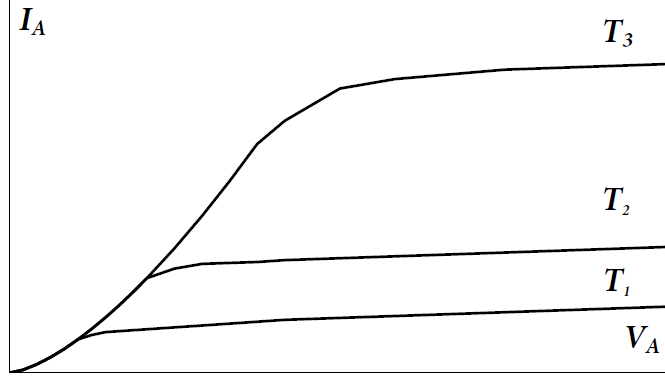
\includegraphics[width=0.5\linewidth]{VAX}
		\caption{ВАХ термоэлектронного диода}
		\label{fig:vax}
	\end{figure}
	
	Потенциальный барьер на границе  металл--вакуум в модели Зоммерфельда характеризуется работой выхода $\varphi$ и средним надбарьерным отражением $\bar{r}$. По формуле Ричардсона-Дэшмана максимальна плотность тока 
	
	\begin{equation}
		j = A_o (1- \bar{r}) T^2 \exp(-\frac{\varphi}{kT})
	\end{equation}
	
	где $A_0 = 120,14$ А/см$^2$К$^2$ - постоянная Зоммерфельда.
	
	В случае, если напряжение на аноде $V_A$ отрицательное, не все электроны смогут преодолеть дополнительный потенциальный барьер (см. рис. 2a):
	
	\begin{equation}
		j = A_o (1- \bar{r}) T^2 \exp(-\frac{\varphi - eV_A}{kT})
	\end{equation}
	
	Если работы выхода катода и анода не совпадают, то ВАХ смещается вправо по оси абсцисс на $(\varphi_K - \varphi_A)/e$ (см. рис. 2b).
	
	При высоких напряжениях работа выхода понижается на $\Delta\varphi = e\sqrt{eE}$ (эффект Шоттки), с учётом чего формула (1) приобретает вид
	
	\begin{equation}
		j = A_o (1- \bar{r}) T^2 \exp(-\frac{\varphi - e\sqrt{eE}}{kT})
	\end{equation}
	
	Т.е. появляется зависимость тока насыщения диода от приложенного к нему напряжения (см. рис. 2c).
	
	\begin{figure}[h!]
		\centering
		\subfloat[]{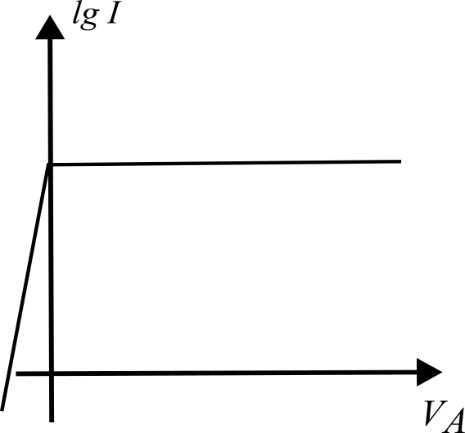
\includegraphics[width=0.25\textwidth]{1}}
		\hfill
		\subfloat[]{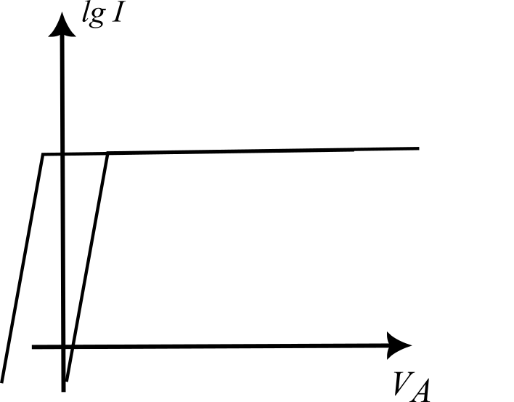
\includegraphics[width=0.3\textwidth]{2}}
		\hfill
		\subfloat[]{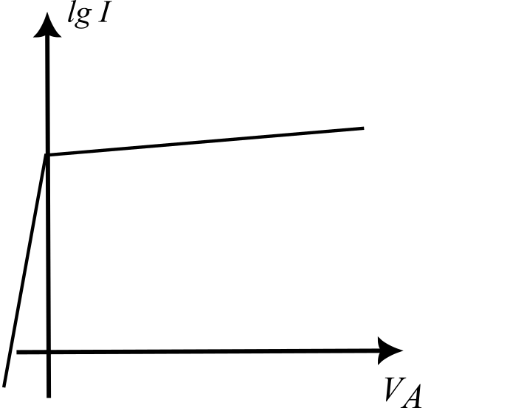
\includegraphics[width=0.3\textwidth]{3}}
		\caption{ВАХ по формуле Ричардсона-Дэшмана}
	\end{figure}
	
	
	При наличии тока эмиссии между катодом и анодом появляется отрицательный пространственный заряд. Поэтому потенциал распределяется нелинейно (см. рис. 3). Пока на этой кривой нет минимума, пространственный заряд не влияет на ток эмиссии. Если же минимум $V_m$ появляется, то ток через диод $I_A$ становится меньше тока насыщения $I_0$:
	
	\begin{equation}
		I_A = I_0 \exp(-\frac{eV_m}{kT})
	\end{equation}
	
	\begin{figure}[h!]
		\centering
		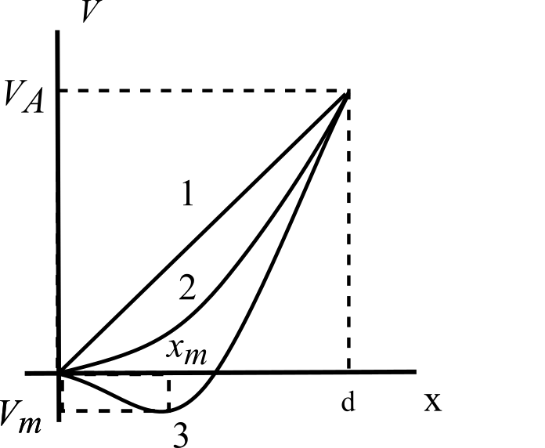
\includegraphics[width=0.5\linewidth]{Vx}
		\caption{Распределение потенциала V(x)}
		\label{fig:vx}
	\end{figure}
	
	
	Заметим, что при больших по величине как положительных, так и отрицательных значениях анодного напряжения объёмный заряд не влияет на ток диода (см. рис. 4). Его влияние на ВАХ представлено на рис. 5 и в упрощённом случае плоскопараллельного диода описывается формулой Чайлда-Ленгмюра
	
	\begin{equation}
		I = \frac{4\sqrt{2}}{9d^2} \sqrt{\frac{e}{m}}S\varepsilon_0 V_A^{\frac{3}{2}} = g V_A^{\frac{3}{2}}
	\end{equation}
	
	где $d$ -- расстояние между анодом и катодом, $S$ -- площадь катодов, $g$ -- первеанс диода.
	
	\begin{figure}[h!]
		\centering
		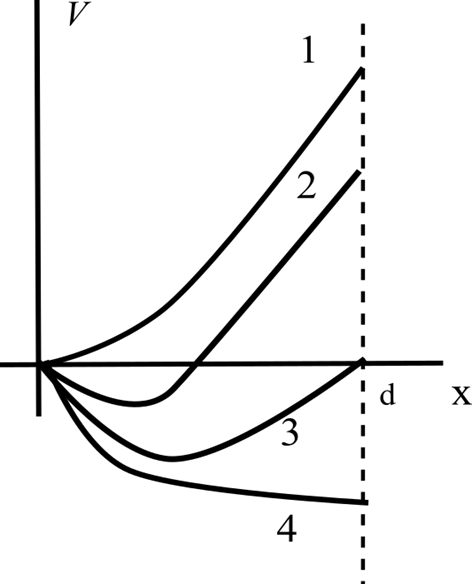
\includegraphics[width=0.3\linewidth]{Vx2}
		\caption{График $V(x)$ при разных $V_A$}
		\label{fig:vx2}
	\end{figure}
	
	
	Для цилиндрической системы с радиусом анода $r$ приближённое выражение для первеанса имеет вид
	
	\begin{equation}
		g = \frac{4\sqrt{2}\varepsilon_0}{9}\sqrt{\frac{e}{m}} \cdot \frac{S}{r^2}
	\end{equation}
	
	\begin{figure}[h!]
		\centering
		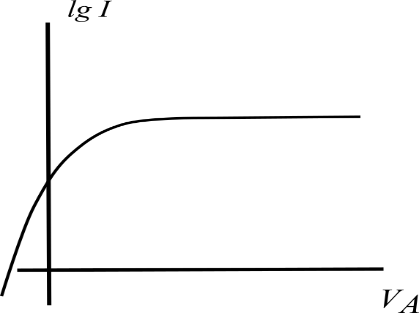
\includegraphics[width=0.5\linewidth]{VAX2}
		\caption{ВАХ диода с учётом объёмного заряда}
		\label{fig:vax2}
	\end{figure}
	
	
	
	
	
	
	
	\section{ОПИСАНИЕ УСТАНОВКИ}
	
		\begin{figure} [h!]
			\centering
			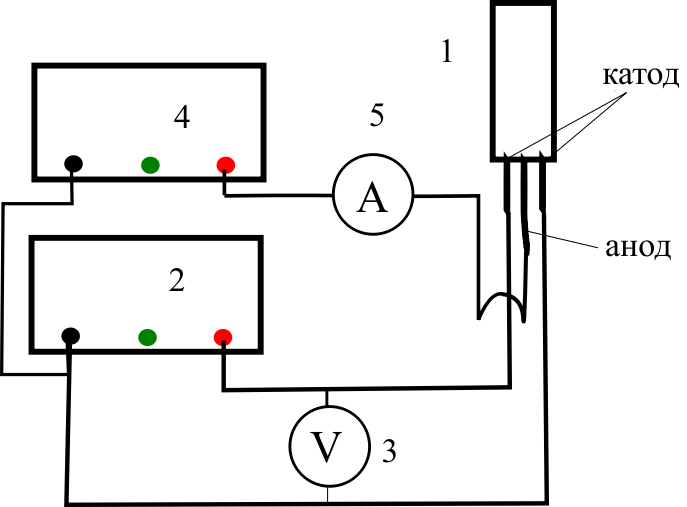
\includegraphics[width=0.5\linewidth]{setup}
			\caption{Упрощённая схема установки: 1 -- диод, 2 -- регулируемый источник тока накала, 3 -- вольтметр, 4 -- регулируемый источник напряжения, 5 -- амперметр.}
			\label{fig:setup}
		\end{figure}
		
		\hspace{5mm} Упрощённая схема установки без вакуумной системы представлена на рисунке \ref{fig:setup}. С использованием вольтметра 3, встроенного в источник 2, измеряется зависимость напряжения накала от тока накала. При достижении значения тока накала 2 А подключается источник 4, на котором устанавливается напряжение от 1 до 60 В. При этом с амперметра 5 снимается ВАХ.
		
		
	\section{ИЗГОТОВЛЕНИЕ ДИОДА} 
	
		\hspace{11mm} Анод изготовлен из никелевого листа толщиной 0,2 мм и шириной 30 мм, намотанного на оправку диаметром 10 мм. Из-за неплотного прилегания диаметр цилиндрического анода принят $d = (11 \pm 1)$ мм.
		
		Катод изготовлен из вольфрамовой проволоки диаметром 0,15 мм. Траверсы -- из никелевой проволоки диаметром 0,8 мм. Использована готовая металлостеклянная ножка.
		
		Монтаж производится при помощи электроконтактной сварки. Схема готового диода представлена на рис. 7.
		
		\begin{figure}[h!]
			\centering
			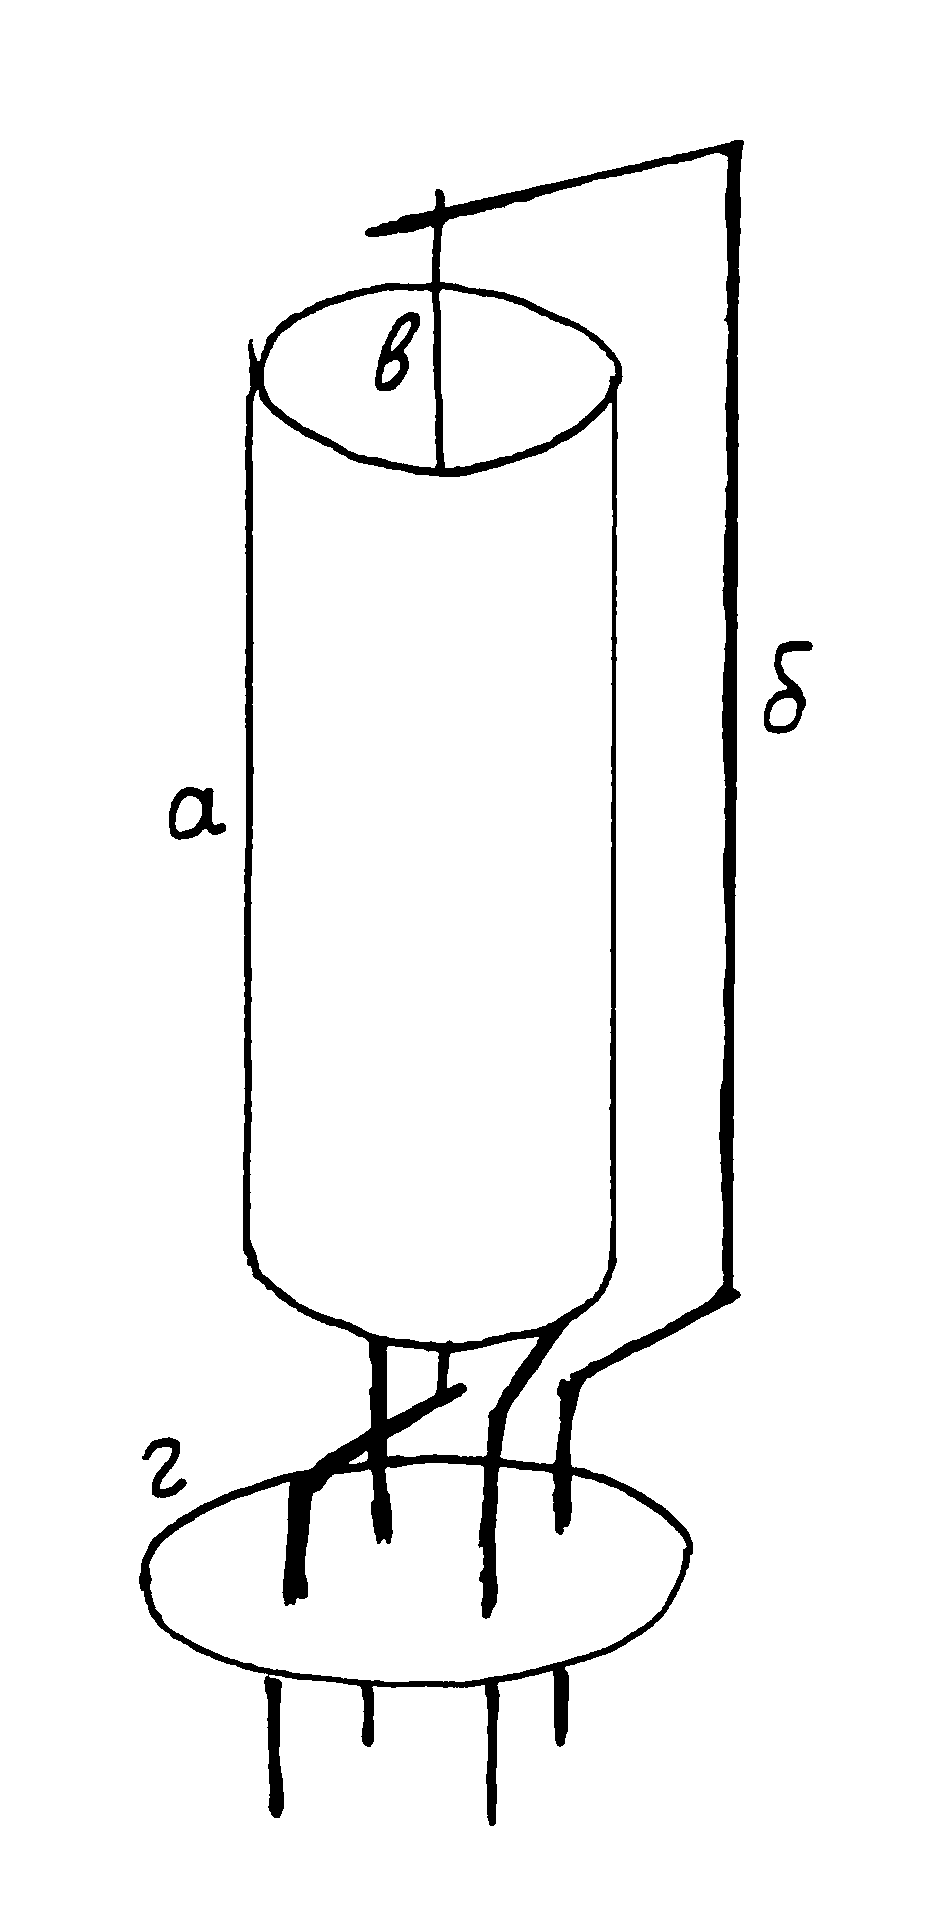
\includegraphics[width=0.3\linewidth]{diode}
			\caption{Схема готового диода: а -- анод, б -- натягивающая траверса, в -- вольфрамовая нить катода, г -- ножка.}
			\label{fig:diode}
		\end{figure}
		
		
		
		
	\section{ХОД РАБОТЫ}
	
	\begin{enumerate}
		
		\item Изготовленный диод помещён в вакуумную установку.
		
		\item Система откачана до $3,7 \cdot 10^{-5}$ Торр.
		
		\item С целью прогрева катода ток накала постепенно поднят до 2,9 А с шагом 0,1 А. Вместе с тем снята зависимость напряжения накала от тока накала.
		
		\item Сняты ВАХ диода в диапазоне анодных напряжений 1 -- 60 В (15 значений с переменным шагом 1, 2 и 5 В) при 6 значениях тока накала в диапазоне 2,4 -- 2,9 А с шагом 0,1 А.
		
		
	\end{enumerate} 
		
	
	\section{РЕЗУЛЬТАТЫ И ОБСУЖДЕНИЯ}
	
	\hspace{11mm} 
	
	
	\section*{ЗАКЛЮЧЕНИЕ}
	\addcontentsline{toc}{section}{ЗАКЛЮЧЕНИЕ}
	
	\hspace{11mm} В ходе выполнения настоящей работы был изготовлен термоэлектронный диод и освоен метод измерения его параметров и характеристик.
	
	В теоретической части рассмотрена простейшая модель термоэлектронного диода. Рассмотрены выражения для анодного тока с учётом эффекта Шоттки и объёмного заряда. 
	
	
	
	Измеренный коэффициент пропускания алюминиевой плёнки $T = 0{,}046 \pm 0{,}002$. По эмпирическим
	данным определена толщина плёнки:
	$h = (25{,}7 \pm 0{,}4)$~нм.
	
	Полученное значение полностью входит в доверительный интервал
	расчётной оценки $(27 \pm 4)$~нм, однако его среднее значение
	несколько ниже расчётного. Занижение обусловлено усреднением толщины
	по области прохождения светового луча, поскольку расчётная толщина
	достигается только в точке, ближайшей к источнику. Дополнительными
	факторами являются анизотропия испарения и рассеяние частиц алюминия
	остаточными газами.
	
	Цель работы достигнута: освоен метод термовакуумного
	напыления тонких плёнок, получена алюминиевая плёнка на стеклянной
	подложке и определена её толщина оптическим методом. 
	
	\section*{СПИСОК ИСПОЛЬЗОВАННЫХ ИСТОЧНИКОВ}
	\addcontentsline{toc}{section}{СПИСОК ИСПОЛЬЗОВАННЫХ ИСТОЧНИКОВ}
	
	\begin{enumerate}
		\item Термоэлектронный диод: лабораторная работа по курсу Вакуумная электроника/ сост. В.М. Агафонов, Е.П. Шешин. -- Москва: МФТИ, 2022. -- 32 с.
	\end{enumerate}
	
	
\end{document}
